
\subsection{Stereolithografisches Drucken}

Zunächst sollen die Grenzen bzgl. lateraler und vertikaler Auflösung eines Stereolithographen (50X, Miicraft) mit einer Pixelauflösung von 30 µm erfasst werden. Dazu werden verschiedene sowohl Single- als auch Multilayer Strukturen gedruckt.

\subsubsection{Preparation des CAD Models}

Mit einer Pixelauflösung des Druckers von \SI{30}{\micro\meter} wurden die Strukturen so modelliert, dass diese an einem \SI{30}{\micro\meter} x \SI{30}{\micro\meter} Raster ausgerichtet sind, damit später beim Druckauftrag der Slicer an die Wänden der Kanäle volle Pixel und im Kanal nicht belichtet. Bei einem Misalignment wird der Kanal teilweise belichtet, somit auch mitpolymerisiert und es bildet sich im Kanal eine feste Struktur, die vermieden werden soll.

\paragraph{Axondioden\\}


\begin{wrapfigure}[11]{r}{.4\textwidth}
\vspace{5pt}
\centering
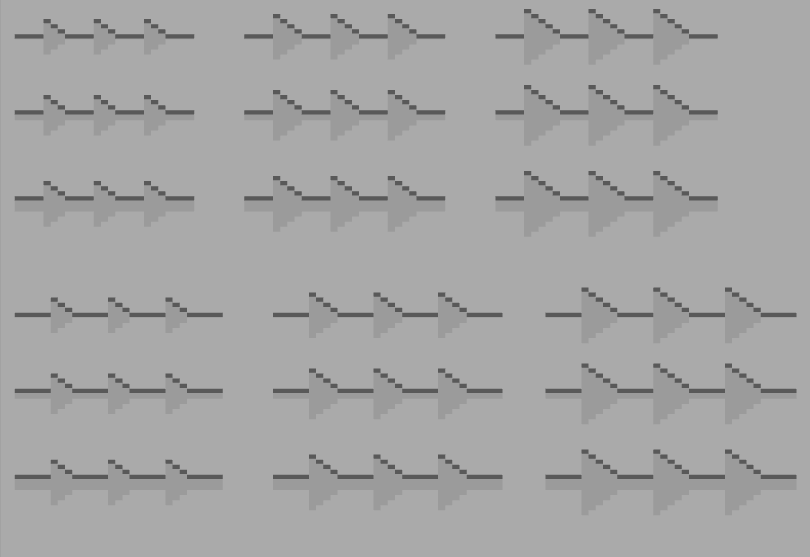
\includegraphics[width=\linewidth]{img/AxonDiode.png}
\caption{Modellierte, pixelausgerichtete Axon-Guiding Strukturen}
\label{fig:AxonDiode}
\end{wrapfigure}

Axondioden werden für Nachbildung von unidirektionalen, synaptischen Verbindungen gebraucht. Hier werden Dreiecke hintereinander gesetzt und mit einem dünnen Kanal verbunden. Dies ist in nebenstehender Abbildung zu erkennen.

Die Dreiecke sorgen dafür, dass nur die Source-Axone von der Hypothenuse des ersten Dreiecks mit Hilfe der beide Katheten wieder zum Kanal und das bis zum Kanal des letzten Dreiecks zum Ziel-Axon schafft. Aus Sicht des Ziel-Axons wird es durch die auseinander laufenden Katheten daran gehindert die Kanäle zu durchlaufen und beim Source-Axon anzukommen.\cite{Gladkov2017}

\paragraph{Wells\\}

Wells sind für Elektroden vorgesehen. Da diese bei rechteckigem Design an den Ecken nicht gut genug belichtet werden und daher eher rund ausfallen, wird außerhalb des Quadrats an jeder Ecke ein weiteres Pixel hinzugefügt, welches mitbelichtet wird und die Struktur letztendlich keine runden Ecken enthält.  

\paragraph{Kanäle\\}

Die Strukturen aus Inventor und Fusion werden dann in Fusion zu einer Datei zusammengeführt und auf eine 3 mm dicke Basis platziert. Es werden Strukturgruppen in vier unterschiedlichen Höhen gedruckt: 10 µm, 25 µm, 50 µm und 100 µm. Die Datei wird darauf als .stl-Datei exportiert und kann an den Drucker weitergegeben werden.

Um die maximale Auflösung des Druckers zu analysieren werden aufgrund der vom Hersteller angegebenen lateralen Auflösung von 30 µm, alle Strukturen in Vielfachen von 30µm-Pixeln realisiert. Bei einer Struktur wird versucht, einen 15 µm breiten Kanal zu konstruieren, indem zwei 30µm-Pixelreihen teilweise belichtet werden und sich in der Mitte der beiden ein dünner Kanal bildet. So werden Kanalbreiten von 30 µm bis 150 µm in 30 µm Schritten erstellt. Auch um 45° gedrehte Kanäle werden gedruckt, um schräge Strukturen zu analysieren. \\

Es soll nicht nur die Auflösung des Druckers erfasst werden, sondern auch welche Layerhöhen verlässlich möglich sind, beispielsweise ob eine 100 µm hohe Struktur besser mit zehn mal 10 µm Layer, vier mal 25 µm oder ein mal 100 µm Layer gedruckt wird und auch, ob eine 10 µm hohe Struktur überhaupt Kanäle frei druckt.

\subsubsection{Durchführung}

Zunächst wird das Reservoir des Druckers mit einem Harz (MedicalPrintClear (MPC) oder eigens gemischter Poly(ethylenglycol) diacrylat (PEGDA) - Lösung) befüllt. PEGDA-Lösung wird mit \SI{2}{\percent} Fotoinitiator Omnirad 2100 (IGM), \SI{0.1}{\percent} UV-absorbierender 5-Benzoyl-4-hydroxy-2-methoxybenzolsulfonsäure (HMBS, Sigma) und \SI{0.01}{\percent} Oxidationsmittel 2,2,6,6-Tetramethylpiperidinyloxyl (TEMPO, Sigma) in PEGDA (mittlere Molmasse 250, Sigma) in einem Ultraschallbad (VWR) gemischt. Die .stl-Datei wird in der Miicraft Software gesliced und mit den gewünschten Druckeinstellungen in eine Mii-Datei konvertiert, die letztendlich zum Druck aufgegeben wird. Die verwendeten Druckeinstellungen waren hierbei (außer anders spezifiziert) \SI{125}{\percent} Leistung und \SI{1}{s} Exposurezeit für Standardlagen, sowie eine Basislage bei einer Exposurezeit von \SI{3}{s}. 

Nach der Fertigstellung wurde ein Skalpell verwendet, um den Druck von dem Picker zu entfernen. Anschließend wurde das gedruckte Objekt mit Isopropanol (99\%, Sigma) abgespritzt und für Zeiten von 5, 10 oder 30 Minuten in Isopropanol in einem Ultraschallbad gereinigt. Am Ende des Prozesses wurde der Druck mit Pressluft getrocknet und in einem Polymerisationsgerät (Otoflash G171) mit 2000 Blitzen unter einer Schutzgasatmosphäre aus Stickstoff ausgehärtet. Dieses strahlt im Wellenlängenbereich von 280 nm - 580 nm mit einer Leistung von 200 Watt. Mit 10 Blitzen pro Sekunde ergibt sich somit eine Belichtungszeit von 3 Minunten und 20 Sekunden bei einer Leistung von 200 W, also idealerweise einer Energie von 11,1 Wh. Optional kann der Druck anschließend im Ofen bei 40°C getrocknet werden, um die restlichen Lösungsmittel aus dem Druck zu verdunsten.


\subsubsection{Oberflächenvermessung}

Für die Oberflächenvermessung der gedruckten Objekte wurde ein konfokales Laser-Mikroskop (Profilometer VK-X 200, Keyence) genutzt. Dazu wurden Bilder optisch und mit dem Laserprofilometer in vorgegebenen Fokuslimits aufgenommen und aneinander gestitcht, um den gesamten Druck später vermessen zu können. Anschließend wurden mittels des Multi-File Analyzers (Keyence) standardisierte, manuelle Messungen von Profiltiefen, teils mit einem Durchschnitt von 5-20 Linien durchgeführt. Das Standardprotokoll bestand sich zum Einen aus der Vermessung aller Kanalstrukturen mittels einer Linie senkrecht zum Kanal mit einem Durchschnitt aus 20 Linien. Zum Anderen wurden die Wells mit verschiedenen Linien angepasst auf deren Größe vermessen (\SI{30}{\micro\meter}: 1 Linie, \SI{60}{\micro\meter}: 2 Linien, ab \SI{90}{\micro\meter}: 5 Linien).

\subsubsection{Silanisierung der Objektträger und Sensoren}

Damit MPC oder PEGDA besser am bzw. überhaupt erst am Objektträger oder Chips hielt, mussten diese zunächst silanisiert werden. Das Silanisierungsprotokoll lief wie folgt ab: \\
\\
1. Ultraschall in purem Toluol für \SI{5}{\minute}; Behälter mit Parafilm verschließen, um Verdunstung zu vermeiden\\
2. Plasmaaktivierung bei \SI{0.8}{\milli\bar} O$_2$ und 100 \% Leistung für \SI{5}{\minute} \\
3. Inkubation im Silan-Lösung für einen Tag; Silan-Lösung wurde aus 5 \% 3-trimethoxysilylpropyl methacrylat (TMSPMA) in Toluol hergestellt; Behälter mit Parafilm verschließen, um Verdunstung zu vermeiden\\
4. Erneut Ultraschall in purem Toluol für 5 Minuten; Behälter mit Parafilm verschließen, um Verdunstung zu vermeiden\\
5. Mehrmals mit dH$_2$O abspülen; gegebenfalls kurz Ultraschall, bis sich weißer Film von Objektträgern löst \\
6. Trocknen mit Pressluft \\
7. Trocknen im Ofen bei 120°C für eine Stunde \\
8. Lagerung im Ofen bei 75°C

\clearpage

\subsubsection{Mikrofluidik}
Zum Design der Mikrofluidik wurden einige theoretische Betrachtungen unter verschiedenen Vereinfachungen getroffen. Verbindungen zwischen den einzelnen Komponenten wurden vernachlässigt und die Dimensionen als ideal angenommen. Als Schlauch wurden jeweils \SI{20}{\centi\meter} Tygon Tubing (Außen - \O{}: 1/16", Innen - \O{}: 1/32") verwendet. Die rechteckige Zu- und Ableitung besitzt jeweils Dimensionen (l x b x h) von \SI{3.7}{\milli\meter} x \SI{1.0}{\milli\meter} x \SI{300}{\micro\meter}. Der Messkanal über dem Sensor misst \SI{8}{\milli\meter} x  \SI{1.0}{\milli\meter} x \SI{300}{\micro\meter}.\\
  
So ergibt nach der Reynoldszahl über dem Flussratensensor mit der Dichte von Wasser $\rho$ = \SI{1000}{\kilo\gram\per\cubic\meter} und einer charakteristischen Kanalbreite $w$ von \SI{1}{\milli\meter} nach (\ref{eq:reynolds}) eine laminare Strömung für Geschwindigkeiten unter \SI{2.3}{\meter\per\second}

\begin{equation}
    \mathit{Re} = \frac{\rho \, v \, w}{\eta}\ <\ 2300 \label{eq:reynolds}
\end{equation}
  

Unter der Vernachlässigung sämtlicher kapazitiver Effekte ergibt sich ein Netzwerk aus rein seriellen Widerständen, für welche Formel (\ref{eq:ohm}) gilt.\cite{Kirby2009} In den folgenden Formel bezeichnen $l$, $w$, $h$ und $r$ jeweils die charakteristischen Dimensionen Länge, Breite, Höhe und Radius. Mit der Beschränkung auf Wasser als Medium ergibt sich die dynamische Viskosität $\eta$ zu \SI{1}{\milli\pascal\second}. Mit geeigneten Annahmen ($h$ < $w$) vereinfacht sich Gleichung (\ref{eq:rect_compl}) zu (\ref{eq:rec_easy}).\cite{TheoreticalMicrofluidics} Mit diesen Gleichungen ergeben sich also $R_{Schlauch}$ zu \SI{1.98e9}{\pascal\second\per\cubic\meter}, $R_{Kanal}$ zu \SI{4.38e9}{\pascal\second\per\cubic\meter} und $R_{Schlauch}$ zu \SI{2.03e9}{\pascal\second\per\cubic\meter}.
 \begin{align}
     Q\ &=\ \frac{\Delta p}{\sum\limits_{Fluss} R} \label{eq:ohm}\\
     \sum\limits_{Fluss} R\ &=\ R_{Schlauch}+ R_{Zulauf} +R_{Kanal} + R_{Ablauf} + R_{Schlauch}\\
     R_{Zulauf}\ &=\ R_{Ablauf} \\
     \sum\limits_{Fluss} R\ &=\ 2\ \cdot\ R_{Schlauch}\ +\ 2\ \cdot\ R_{Zulauf}\ +\ R_{Kanal}\\
     R_{Schlauch}\ &=\ \frac{8\eta l}{\pi r^4}\ =\ \frac{8\cdot\SI{1}{\milli\pascal\second} \cdot \SI{200}{\milli\meter}}{\pi \cdot \SI{1.58}{\milli\meter}^4}\ =\ \SI{8.17e7}{\pascal\second\per\cubic\meter} \\
     R_{Kanal, Zulauf}\ &=\ \frac{12 \eta l}{w\ h^3}\ \left[1-6 \left(\frac{h}{w}\right) \sum\limits_{n=0}^{\infty} \left( \frac{(2n+1)\pi}{2} \right)^{-5} \tanh{ \left( \frac{(2n+1)\pi\ w}{2\h} \right) } \right]^{-1} \label{eq:rect_compl}\\
     R_{Kanal, Zulauf}\ &\approx \frac{12 \eta l}{w h^3(1-(0.630h)/w)} \label{eq:rec_easy} 
 \end{align}
 Daher ergibt sich folgende Relation für die Flussrate abhängig vom angelegten Druck:
 \begin{equation}
     Q(\Delta p) = \frac{\Delta p}{\SI{1.10e10}{\pascal\second\per\cubic\meter}}
 \end{equation}